\begin{wrapfigure}{r}{0.5\textwidth}
	\begin{center}
	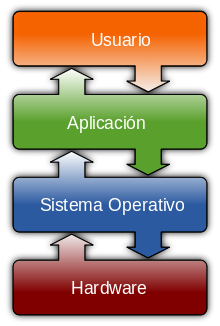
\includegraphics[width=0.2\textwidth]{./debuxos/capas.png}
	 \caption{Situación do sistema operativo}
	 \end{center}
	 \label{capas}
\end{wrapfigure}

\begin{doublespace}
Nos anos corenta cando se comezaron a construír ordenadores os programadores tiñan que ter en conta as peculiaridades do equipo co que traballaban. Non era o mesmo programar para un procesador ou para outro, as instrucións tiñan que indicar por exemplo o espacio de memoria que se ía usar. Co paso do tempo foron decatándose de que era mellor ter un software que se ocupara dos detalles de máquina e que o programador poidera executar o seu código en calquera equipo. Precisaban un software que se encargara dos detalles concretos do ordenador: do espacio libre en memoria, das instrucións que variaban dun procesador a outro, de verificar se todo funcionaba correctamente,... Paseniño foise creando ese software que permite ó programador ocuparse do seu cálculo ou do seu algoritmo sen ter que preocuparse en que parte da memoria se executa ou cal é o procesador que lle está resolvendo as súas contas. 

Un sistema operativo é ese conxunto de programas que actúan coma intermediario entre o usuario e o hardware do ordenador. Na figura \ref{capas} vemos como o sistema operativo sitúase facendo de intermediario entre os dispositivos físicos e as aplicacións de usuario.\\
\end{doublespace}

\begin{diapo} \begin{frame}{Un sistema operativo é  \dots} 
\begin{enumerate}
\item hardware\pause
\item software \pause
\item malware 
\end{enumerate}
\end{frame} 
\end{diapo} 
%parella
\begin{diapo}\begin{frame}{Os que xestionan o hardware son  \dots}
\begin{enumerate}
\item drivers \pause
\item terminais \pause
\item sistemas operativos
\end{enumerate}
\end{frame}
\end{diapo}

